\section{From local covariances to the momentum distribution}
\label{mom:section}\label{sec:momentum}

The local covariance estimate describes one-body operators inside a
$B$-box, whereas momentum occupation is defined by Fourier modes on the
whole torus. Translations connect these two descriptions: their
expectations are the Fourier transform of the momentum measure. We
first remove the remaining cell-constant excitations, then average the
position of the $B$-box boundaries. This makes the cost of cutting a
translation small compared with the excitation count.

\subsection{Translations and shifted box boundaries}

For a normalized ground vector $\Phi$ on $\Lambda_K$, put
$u_{p,K}(y)=V^{-1/2}e^{ip\cdot y}$ and define the positive momentum measure
\begin{equation}\label{mom:scaled-measure}
 \mathfrak m_\Phi
   =\frac1V\sum_{\substack{p\in(2\pi/K)\Z^3\\p\ne0}}
       \langle u_{p,K},\gamma^{(1)}_\Phi u_{p,K}\rangle\,\delta_p.
\end{equation}
Here $\gamma^{(1)}_\Phi$ is the one-particle density matrix of $\Phi$ and
$\delta_p$ is unit mass at $p$. Let $T_hg(y)=g(y+h)$ for $h\in\R^3$.
Since $T_hu_{p,K}=e^{ih\cdot p}u_{p,K}$,
\begin{equation}\label{mom:translation-identity}
 \int e^{ih\cdot p}\,\dd\mathfrak m_\Phi(p)
   =\frac1V\langle\dd\Gamma((1-P_0)T_h(1-P_0))\rangle_\Phi.
\end{equation}

Recall $Q_R=P_R-P_0$ and $1-P_0=W_R+Q_R$. The inputs from
\eqref{en:R-occupation} and Proposition~\ref{asm:infrared} give
\begin{equation}\label{mom:excitation-masses}
 a_\Phi:=\frac1V\langle\dd\Gamma(W_R)\rangle_\Phi=O(1),
 \qquad
 b_\Phi:=\frac1V\langle\dd\Gamma(Q_R)\rangle_\Phi=o(1).
\end{equation}
For the second assertion, the operators and exponents can be held fixed
as $j$ increases; one chooses $j$ first and the dilution threshold
afterward. Both assertions are uniform over all complex ground vectors.
Expanding \eqref{mom:translation-identity} and applying Cauchy--Schwarz
to the sum over particles yields
\begin{equation}\label{mom:remove-coarse}
 \left|\int e^{ih\cdot p}\,\dd\mathfrak m_\Phi(p)
       -\frac1V\langle\dd\Gamma(W_RT_hW_R)\rangle_\Phi\right|
       \le b_\Phi+2\sqrt{a_\Phi b_\Phi}=o(1).
\end{equation}
This bound is uniform in $h$. In particular, the subsequent boundary
estimate will be multiplied by $a_\Phi$, the excitation density.

Fix $H<\infty$. Keep the $R$-grid fixed and let $\mathcal S$ be the
family of $B$-box partitions obtained by shifting the original grid by
\[
 \theta\in\{0,R,\ldots,B-R\}^3.
\]
Every partition in this family is still a union of the same $R$-cells.
For $\mathcal C\in\mathcal S$ define the translation cut at its box faces by
\begin{equation}\label{mom:cut-translation}
 T_h^{\mathcal C}=\sum_{b\in\mathcal C}\1_bT_h\1_b.
\end{equation}
The average below is the uniform average over $\mathcal S$.

\begin{lemma}[Averaging box boundaries]\label{mom:shift-average}
If $K>2(B+H)$ and $|h|\le H$, then
\begin{equation}\label{mom:shift-norm}
 \left\|T_h-\operatorname{Avg}_{\mathcal C\in\mathcal S}
                        T_h^{\mathcal C}\right\|
          \le C\frac{H+R}{B}.
\end{equation}
\end{lemma}

\begin{proof}
For fixed $y$, the difference is $T_h$ followed by multiplication by
the fraction of partitions that put $y$ and $y+h$ in different boxes.
In one coordinate, separation requires a box face between the two
lifted coordinates. As the shift varies, possible faces are spaced by
$R$, so at most $H/R+2$ of the $B/R$ shifts separate the pair.
A union bound over the three coordinates proves the uniform multiplier
bound \eqref{mom:shift-norm}. The count also applies across the periodic
boundary; the stated restriction on $K$ allows the interval to be
lifted without ambiguity. Cell faces themselves are null sets.
\end{proof}

Figure~\ref{fig:shifted-grid} illustrates why the averaging is uniform in
the position of the translated pair. Because $R/B\to0$ and $B\to\infty$,
Lemma~\ref{mom:shift-average} and \eqref{mom:excitation-masses} imply
\begin{equation}\label{mom:boundary-cost}
 \left|\frac1V\langle\dd\Gamma(W_RT_hW_R)\rangle_\Phi
  -\operatorname{Avg}_{\mathcal C\in\mathcal S}
      \frac1V\langle\dd\Gamma(W_RT_h^{\mathcal C}W_R)\rangle_\Phi\right|
       \le C\frac{H+R}{B}\,a_\Phi=o(1).
\end{equation}
The number of shifted grids creates no additional factor in this estimate.
The replacement of the full particle density $D$ by $a_\Phi$ is
essential, since $D(H+R)/B$ does not tend to zero at the chosen scales.

\begin{figure}[tb]
 \centering
 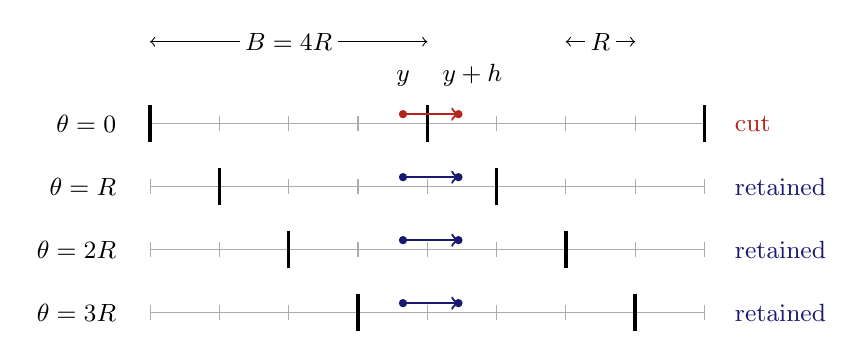
\begin{tikzpicture}[x=.88cm,y=.8cm,font=\small]
 \foreach \row/\shift/\name in {0/0/{0},1/1/{R},2/2/{2R},3/3/{3R}} {
  \begin{scope}[yshift=-\row*0.8cm]
   \node[anchor=east] at (-.35,0) {$\theta=\name$};
   \draw[gray!65] (0,0)--(8,0);
   \foreach \x in {0,...,8} {\draw[gray!65] (\x,-.12)--(\x,.12);}
   \ifnum\row=0
    \foreach \x in {0,4,8} {\draw[very thick] (\x,-.29)--(\x,.29);}
    \draw[->,thick,BrickRed] (3.65,.15)--(4.45,.15);
    \fill[BrickRed] (3.65,.15) circle (1.5pt);
    \fill[BrickRed] (4.45,.15) circle (1.5pt);
    \node[anchor=west,BrickRed] at (8.3,0) {cut};
   \else
    \draw[very thick] (\shift,-.29)--(\shift,.29);
    \draw[very thick] (\shift+4,-.29)--(\shift+4,.29);
    \draw[->,thick,MidnightBlue] (3.65,.15)--(4.45,.15);
    \fill[MidnightBlue] (3.65,.15) circle (1.5pt);
    \fill[MidnightBlue] (4.45,.15) circle (1.5pt);
    \node[anchor=west,MidnightBlue] at (8.3,0) {retained};
   \fi
  \end{scope}
 }
 \node[anchor=south] at (3.65,.43) {$y$};
 \node[anchor=south] at (4.65,.43) {$y+h$};
 \draw[<->] (0,1.3)--(4,1.3);
 \node[fill=white,inner sep=2pt] at (2,1.3) {$B=4R$};
 \draw[<->] (6,1.3)--(7,1.3);
 \node[fill=white,inner sep=2pt] at (6.5,1.3) {$R$};
\end{tikzpicture}

 \caption{A one-dimensional section of the shifted partitions, with
 $B=4R$ and a fixed pair $y,y+h$. Thin ticks mark the same $R$-grid in
 every row; thick ticks are the $B$-box faces. In the first row the
 translation crosses a box face and is cut. In the other three rows it
 stays inside one box. In general, only $O(H/R+1)$ of the $B/R$ shifts
 can separate a pair with $|h|\le H$. Sandwiching the averaged error
 by $W_R$ makes its expectation cost proportional to the excitation
 density, as in \eqref{mom:boundary-cost}.}
 \label{fig:shifted-grid}
\end{figure}

\subsection{The Fourier transform of the limiting density}

Each cut translation acts separately on the $B$-boxes. We may therefore
apply Proposition~\ref{mom:local-covariance} to it. The remaining
calculation identifies the Neumann-mode trace with the Fourier transform
of $F_\alpha$, defined in \eqref{en:limiting-V}.

\begin{proposition}[Momentum characteristic integrals]
\label{mom:characteristic}
For every fixed $H<\infty$,
\begin{equation}\label{mom:characteristic-limit}
 \int e^{ih\cdot p}\,\dd\mathfrak m_\Phi(p)
     =\int_{\R^3}e^{ih\cdot p}F_\alpha(p)
                          \frac{\dd p}{(2\pi)^3}+o(1),
 \qquad |h|\le H.
\end{equation}
The error is uniform in $h$ and in normalized, possibly complex,
ground vectors, with the iterated-limit convention of
Section~\ref{set:section}.
\end{proposition}

\begin{proof}
Fix a shifted partition $\mathcal C$. In local coordinates $[0,B)^3$,
the restriction of $T_h^{\mathcal C}$ is the contraction
\[
 (C_{b,h}g)(y)=\1_{[0,B)^3}(y+h)g(y+h).
\]
It is identical in every box. Write $W$ for the restriction of $W_R$
to a box, and $e_p$ for its normalized Neumann cosine mode with
$p\in(\pi/B)\N_0^3$. Proposition~\ref{mom:local-covariance}, including
its complex-contraction assertion, gives
\begin{equation}\label{mom:local-translation-trace}
 \frac1V\langle\dd\Gamma(W_RT_h^{\mathcal C}W_R)\rangle_\Phi
  =\frac1{B^3}\sum_{p\ne0}
        \langle e_p,WC_{b,h}We_p\rangle F_\alpha(p)+o(1).
\end{equation}
The estimate applies uniformly to these shifted grids: simultaneous
translation maps the ground space unitarily to itself, and the local
bound is uniform over its normalized vectors.

We compute the diagonal on a fixed annulus
$0<\delta\le|p|\le J$. At least one coordinate has
$|p_i|\ge\delta/\sqrt3$. The mean of its cosine over an $R$-interval
is bounded by $2/(R|p_i|)$, whereas each other cosine mean has absolute
value at most one. Including the Neumann normalization factors and
summing the squared cell means gives
\[
 \|(1-W)e_p\|\le\frac{C}{\delta R}.
\]
Since $C_{b,h}$ is a contraction,
\begin{equation}\label{mom:Neumann-diagonal}
 \langle e_p,WC_{b,h}We_p\rangle
   =\prod_{i=1}^3\cos(p_i h_i)
                  +O\left(\frac1{\delta R}+\frac HB\right).
\end{equation}
To verify the translation term, extend the cosine formula for $e_p$
to $\R^3$. Removing the clipping changes its integral by $O(H/B)$:
the boundary layer has relative volume $O(H/B)$ and
$|e_p(y)e_p(y+h)|\le C/B^3$. On the full box the integral factors.
For $p_i>0$, the sine--cosine integral over $[0,B]$ is zero because
$p_iB\in\pi\N$; the cosine-square integral gives $\cos(p_i h_i)$.
For $p_i=0$ the factor is one.

Uniformly for $\alpha\in I_\alpha$, the explicit formula gives
\begin{equation}\label{mom:profile-majorant}
 F_\alpha(p)\le C\min(|p|^{-1},|p|^{-4}).
\end{equation}
The normalized Neumann-lattice tails in \eqref{en:lattice-tails}
therefore bound the contributions of $0<|p|\le\delta$ and $|p|\ge J$
by $C\delta^2$ and $C/J$, respectively, uniformly in $B$, for
$0<\delta<1<J$. The same bounds hold for the corresponding integrals.

We can now truncate \eqref{mom:local-translation-trace} to a fixed
annulus, use \eqref{mom:Neumann-diagonal}, and take Riemann sums.
The Neumann mesh has density $\pi^{-3}$ in the nonnegative octant.
On the annulus the integrands are bounded and equicontinuous for
$|h|\le H$ and $\alpha\in I_\alpha$; continuous cutoffs at its edges
may be used. Letting $\delta\downarrow0$ and $J\uparrow\infty$ after
these estimates yields, uniformly in $h$ and $\mathcal C$,
\begin{align}
 \frac1V\langle\dd\Gamma(W_RT_h^{\mathcal C}W_R)\rangle_\Phi
 &=\frac1{\pi^3}\int_{[0,\infty)^3}
       F_\alpha(p)\prod_i\cos(p_i h_i)\,\dd p+o(1)\notag\\
 &=\int_{\R^3}F_\alpha(p)e^{ih\cdot p}
                          \frac{\dd p}{(2\pi)^3}+o(1).
 \label{mom:octant-Fourier}
\end{align}
The last equality uses reflection symmetry in each coordinate.
Averaging over $\mathcal C$ and applying
\eqref{mom:remove-coarse} and \eqref{mom:boundary-cost} proves
\eqref{mom:characteristic-limit}.
\end{proof}

\subsection{Physical units and bounded continuous tests}

The characteristic integrals include the total mass by taking $h=0$.
Fourier inversion will first give compact-test convergence. Together
with total mass convergence and positivity, this controls the momentum
tails and allows arbitrary bounded continuous test functions.

\begin{proof}[Proof of Theorem~\ref{thm:main}]
Fix $a>0$. For a sufficiently small density $\rho>0$, put
$\eta=\rho a^3$ and
\begin{equation}\label{asm:physical-scale}
 s_* =\sqrt{\frac{\alpha_0}{\rho a}},\qquad
 D_* =\rho s_*^3=\frac{\alpha_0^{3/2}}{\sqrt\eta}.
\end{equation}
Choose $R,B$ from this $D_*$ by \eqref{set:nested-lengths}.
For any thermodynamic sequence $N_k,L_k\to\infty$ with
$N_k/L_k^3\to\rho$, let $K_k$ be a positive multiple of $B$ nearest
to $L_k/s_*$. Set
\[
 s_k=L_k/K_k,\qquad r_k=a/s_k,\qquad
 D_k=N_k/K_k^3,\qquad \alpha_k=D_kr_k.
\]
Then $K_k\to\infty$, $s_k\to s_*$, $D_k\to D_*$, and
$\alpha_k\to\alpha_0$. Thus all the nested partitions and parameter
conditions hold on the tail of every such sequence.

The unitary change of variables is
\begin{equation}\label{asm:unitary-scaling}
 (U_k\Psi)(y_1,\ldots,y_{N_k})
       =s_k^{3N_k/2}\Psi(s_ky_1,\ldots,s_ky_{N_k}).
\end{equation}
It maps the allowed sets and form domains to their scaled versions,
with $q_{K_k,r_k}[U_k\Psi]=s_k^2q_{L_k,a}[\Psi]$, and hence maps
ground eigenspaces unitarily. The corresponding one-particle unitary
sends a physical plane wave of momentum $\kappa$ to the scaled one
of momentum $p=s_k\kappa$, preserving its occupation. Also
\begin{equation}\label{asm:gas-identity}
 D_kr_k^3=(N_k/L_k^3)a^3\longrightarrow\eta,
 \qquad D_k\sqrt\eta\longrightarrow\alpha_0^{3/2}.
\end{equation}

Suppress $k$ temporarily. For a normalized physical ground vector
$\Psi$, put $\Phi=U\Psi$ and
\begin{equation}\label{mom:physical-measure}
 \lambda=s\sqrt{8\pi\rho a},\qquad
 \sigma_\Psi=\frac1{D\sqrt\eta}
                  (p\mapsto p/\lambda)_*\mathfrak m_\Phi.
\end{equation}
The normalized momentum sum in \eqref{intro:main-limit}, evaluated in
the pure state $|\Psi\rangle\langle\Psi|$, is
$\int f\,\dd\sigma_\Psi$. In the inner limit,
$\lambda\to\lambda_0:=\sqrt{8\pi\alpha_0}$.
The target measure $\sigma_0:=\nu_{\mathrm{Bog}}$ from
\eqref{intro:profile} satisfies
\begin{equation}\label{mom:target-measure}
 \sigma_0=(p\mapsto p/\lambda_0)_*
       \left(\alpha_0^{-3/2}F_{\alpha_0}(p)
                                    \frac{\dd p}{(2\pi)^3}\right).
\end{equation}
This follows by substituting $p=\sqrt{8\pi\alpha_0}\,t$ in the
explicit formula \eqref{en:limiting-V}.

Apply Proposition~\ref{mom:characteristic} at $h/\lambda$ and use
\eqref{asm:gas-identity}. Since $\lambda$ stays bounded away from
zero, we obtain
\begin{equation}\label{mom:physical-characteristic}
 \int e^{ih\cdot t}\,\dd\sigma_\Psi(t)
       =\int e^{ih\cdot t}\,\dd\sigma_0(t)+o(1),
\end{equation}
uniformly on each compact set of $h$ and uniformly over the ground
vectors. Replacing $\alpha,\lambda$ in the continuous integral by
their inner limits costs only an inner-limit error: the majorant in
\eqref{mom:profile-majorant} is integrable, and truncation in $p$ makes
this replacement uniform on compact $h$-sets. The case $h=0$ gives
total mass convergence and, in particular, a uniform mass bound in
the iterated limit.

For $g\in C_c^\infty(\R^3)$, Fourier inversion and its integrable
Fourier transform imply
\[
 \int g\,\dd(\sigma_\Psi-\sigma_0)=o(1).
\]
Indeed, on a fixed compact Fourier set use
\eqref{mom:physical-characteristic}; on its complement use the mass
bound times the $L^1$ tail of the Fourier transform. Uniform
approximation and the same mass bound give this conclusion for all
$g\in C_c(\R^3)$.

Now let $f$ be any bounded continuous real function. Choose
$\chi\in C_c^\infty(\R^3)$ with $0\le\chi\le1$ and
$\int(1-\chi)\,\dd\sigma_0$ as small as desired. Positivity gives
\begin{align}
 \left|\int f\,\dd(\sigma_\Psi-\sigma_0)\right|
 &\le\left|\int f\chi\,\dd(\sigma_\Psi-\sigma_0)\right|\notag\\
 &\quad+\|f\|_\infty\left\{
       2\int(1-\chi)\,\dd\sigma_0
       +|\sigma_\Psi(\R^3)-\sigma_0(\R^3)|
       +\left|\int\chi\,\dd(\sigma_\Psi-\sigma_0)\right|\right\}.
 \label{mom:tightness}
\end{align}
The compact tests and the mass difference tend to zero in the stated
iterated sense. For a prescribed $\eps>0$, first choose $\chi$ and
the compact-test approximations, then choose the auxiliary parameters
and a lower threshold on $D_*$. Equation~\eqref{asm:physical-scale}
turns that threshold into $\rho_0(a,f,\eps)>0$. It works for every
fixed $0<\rho<\rho_0$ and every density-convergent thermodynamic
sequence. The volume threshold may depend on that fixed density and
sequence; no convergence rate for $N_k/L_k^3$ is required.

Finally, Lemma~\ref{set:ground-space} makes every finite-volume ground
eigenspace finite dimensional. Each state in $\mathcal G_{N,L,a}$
has a spectral decomposition
$\Gamma=\sum_b\omega_b|\Psi_b\rangle\langle\Psi_b|$ with
normalized ground vectors, $\omega_b\ge0$, and $\sum_b\omega_b=1$.
Its momentum measure is $\sum_b\omega_b\sigma_{\Psi_b}$. The absolute
error for $f$ is therefore at most the largest pure-state error at
that volume. All preceding bounds were uniform in the pure ground
vector, so the conclusion holds with the supremum over
$\Gamma\in\mathcal G_{N,L,a}$ required by the theorem.
\end{proof}
